%begin-include
In this chapter we present the development process and implementation
details of the SigNetMS software, which stands for {\bf Sig}naling 
{\bf Net}work {\bf M}odel {\bf S}election. This software is capable of
producing an estimative of the marginal likelihood of a model given
experimental data, using the ideas of Thermodynamic Integration. Besides
implementation details, in this chapter we also present the main 
difficulties of creating a computationally efficient implementation of
this software, and also how we tackled these difficulties. 

In order to support some of our implementation choices and also to
explore limitations of our software, a few experiments were performed
and are shown in this chapter. All the experiments of this chapter were
conduced in a server with an Intel Xeon E5-2690 CPU, and 252GB of RAM
memory.

% What are we going to talk about in this chapter?
% - first, we have to talk about which methodology this software uses
%   -> make sure you citate BioBayes and how its cumbersome to use it
% to create a model ranking. we should state that we are using marginal
% likelihood estimates here.
%   -> make sure we specify the input and output of this software
%   -> include program arguments
% - then, we can talk about the implementation and optimizations
%   -> how did we implement the sampling? what was the used proposal
%   distribution?
%   -> fast integration of system of differential equations
%   -> parallel sampling
%   -> running the algorithm on a cluster

\section{The SigNetMS software}
% General Aspects of the software

% The Bayesian methodology
% - SigNeMS creates an estimative of the marginal likelihood of a model
% given a set of experimental data.
% - To create this estimative, SigNetMS uses ideas of Thermodynamic
%   Integration.
% - There is a software that can carry similar simulations, called
%   BioBayes, however we found its use cumbersome, mainly because:
%   it is a GUI software, which does not fit our type of applications,
%   that should be ran in a server for several hours. Moreover, we
%   intended to link the marginal likelihood output to other programs,
%   for model selection.

% Details on how the program creates the system of ODEs
% Details on how the proram estimates the likelihood

SigNetMS is a Python program that can be used as a tool for model
selection, producing an estimative of the marginal likelihood of a model
given experimental observations. The source code is available on 
Github\footnote{https://github.com/gustavoem/SigNetMS} and it is open
source, under the GNU General Public License.

This program expects as the input: a signaling pathway model,
represented by a Systems Biology Markup Language
(SBML)~\cite{hucka2003systems} file, with the definition of reactions,
kinetic laws and initial concentrations of chemical species; an
Extensible Markup Language (XML) file with experimental data, including 
time series measurements of the  biological phenomena of interest;
another XML file with definitions of prior distributions of reaction
rate constants; and, finally, a set of parameter values that determine
the sampling process of model parameters. There are also optional
parameters on SigNetMS, used to control random number generator seeds,
number of execution threads, and verbose runs.

The output of the program is composed by an estimative of the marginal
likelihood of the model, given experimental data, $p({\bm D} | M)$ and a
list of parameter values $({\bm \theta}^1, {\bm \theta}^2, \ldots {\bm
\theta}^l)$ that represent a sample of the distribution $p({\bm \theta}
| M, {\bm D})$. If one simulates the model $M$ with parameter values
from the sample, we expect that, the higher the marginal likelihood, the
closer the created simulation are to the experimental data.

To calculate the marginal likelihood estimative, we use the ideas of 
Thermodynamic Integration we presented on 
section~\ref{sec:thermodynamic_integration}. Before implementing
SigNetMS we also considered using another software, called
BioBayes~\cite{Vyshemirsky2008}, that has a very similar approach to
produce an estimative of the marginal likelihood. However, we did not
proceed to use this software because there was only a graphical user
interface version of the software, which made the process of running
instances and collecting results cumbersome. We have also tried
contacting the authors to obtain the source code, however they could not
provide us that.

\section{Creating an estimative of the marginal likelihood}
\label{sec:creating_an_estimative_of_the_marginal_likelihood}
% Since we are using a Thermodynamic Integration  approach, we need to 
% define a likelihood function, create samples of power posterior 
% distributions and, finally define an approximation to the marginal
% likelihood.

% The likelihood function...
% The samples of power posteriors are...
% The approximation of the marginal likelihood are...
% The whole process, has the following order:
% -> all inputs are read;
%   -> The sbml model is read and transformed into a System of ODE
%       -> this model can determine a simulation, given a list of
%       parameter values and a measurement unit;
%   -> Parameter priors, experimental data are read and saved
% -> sampling of posterior starts with naive sampling
% -> then we proceed to covariance shaped burn-in
% -> then we go to populational monte carlo markov chain
% -> then we use the approximation to generate the margginal likelihood

To create estimates of the marginal likelihood using the Thermodynamic
Integration approach, we need to define a likelihood function $p({\bm
D}| M, {\bm \theta})$ and also samples power posterior distributions
$p_\beta({\bm \theta})$ for a sequence of values of $\beta$. After
samples are produced, we use them to produce the estimative, and on
SigNetMS, we use the trapezoidal rule to approximate the marginal 
likelihood, given by the 
equation~\ref{eq:marginal_likelihood_trapezoidal_approximation}. 
Inspired by the work of Friel et al., we discretize the interval 
$[0, 1]$ of power posteriors using the schedule: 
$\beta_i = \left(\frac{i - 1}{T - 1}\right)^c$, where $T = 20$, $c = 4$
and $i \in \{1, 2, \ldots, T\}$. In the following sections, we explain
how we implemented the likelihood function, and how samples of power
posteriors are produced.

\subsection{Implementing the likelilhood function}
%-> The likelihood function is...
%-> To implement this, we must simulate the model with parameter values
%of theta.
%-> these simulations involves the numerical integration of a system of 
% ordinary differential equaitons
%-> current methods of numerical integrations are iterative and can be
% very consty depending on the size of the numerical system and also on
% the type of the system, stiff or not
The likelihood function we used is the same as we defined in
equation~\ref{eq:likelihood_multivariate}:
\begin{equation*}
    p ({\bm D} | M,{\bm \theta}) = 
        p_{\mathcal{N}_{\left(\vec{0}, \Sigma\right)}}
        (\phi (M, {\bm\theta}) - {\bm D}),
\end{equation*}
where ${\bm D}$ is the experimental measurement, $M$ is the model,
${\bm \theta}$ is a set of parameter values, $\Sigma$ is the variance of
the error of experimental observations, and, finally, $\phi$ is a 
function that calculates an approximation of the results of the
experiment that produced ${\bm D}$, applied to the simulated environment
of model $M$ with parameter values ${\bm \theta}$. This simulation of
the model is created by deriving a system of ordinary differential
equations, and then numerically integrating this system, over the time
steps defined by the experimental measurements. To reproduce the same
experiment that generated ${\bm D}$, SigNetMS expects that the XML file 
containing experimental data also contains a mathematical representation
of which quantity was measured, in terms of concentrations of chemical
species of the system.

% Numerical integration of systems are solved using iterative methods
% stiff non stiff
% we used  third-party software to solve this problem
The numerical integration of the system is alone a hard problem, and
therefore, we used third-party software to produce such integrations.
The most popular software available for this problem conduce
iterative algorithms that, step by step, approximate the state of the
system for a time interval. It is important to know that some instances
of the problem can be stiff, meaning that they may make the integration
algorithm be unstable, since it may need consecutive iterations with
really small steps. Since we did not have time to go in details of when 
such cases occur, we chose third-party software that can adapt the used
algorithm according to the stiffnes of the instance.

After the implementation of the function $\phi$, most of the work to
implement the likelihood function is done. The remaining work is to
calculate the value of the probability density function
$p_{\mathcal{N}_{\left(\vec{0}, \Sigma\right)}}$ and that can easily be
accomplished using statistical packages such as
SciPy~\cite{2020SciPy-NMeth}.

\subsection{Sampling parameters from power-posteriors}
% after implementing the likelihood function, we can create the samples
% of the power posteriors;
% -> we used the same methodology we presented before, this methodology
%  is based on using variations of the metropolis-hastings algorithm,

After implementing the likelihood function, we can move to the creation
of samples of power posteriors. The methodology we used to generate such
samples is identical to the one we presented on
section~\ref{sec:estimation_of_marginal_likelihood}. And for this
reason, we divided the sampling process in three phases: naive burn-in,
adaptive burn-in and Populational MCMC; all of them are types of a 
Metropolis-Hastings procedure. The number of iterations of each phase is
determined by SigNetMS's arguments, and each phase has a different 
scheme to determine the proposal distribution.

On the first phase, we start the sample of every chain (for each value
of $\beta$) with a random draw from the prior distribution of
parameters. Before the first iteration, we also create an estimative of
the variance of the logarithm of each model parameter, independently.
These estimates compose the first covariance matrix of the jumping 
distribution; we use a diagonal matrix where the diagonal elements are
set as the estimated variance of the logarithm scaled sample of the
associated parameter. This matrix is rescaled according to the
acceptance rate, as described in
section~\ref{sec:estimation_of_marginal_likelihood}, after a number of
iterations that is defined in one of the arguments of SigNetMS. For each
iteration, we determine that the jumping distribution is a multivariate
lognormal $({\bm \mu}, \Sigma)$ distribution, with covariance matrix as
explained before, and with ${\bm \mu} = \log_e({\bm \theta}^t)$, where
${\bm \theta}^t$ is the current sample point, i.e., we take a
sample ${\bm X}$ of the multivariate normal $\mathcal{N}({\bm \mu},
\Sigma)$ and then we set our sampled value  as ${\bm Y} = \exp({\bm
X})$, which is a standard procedure to produce samples of lognormal
distributions.

On the second phase, the posterior shaped burn-in phase, we also use a 
lognormal as the proposal distribution, however the covariance matrix is 
not diagonal. Half of the sample produced in the first phase is
discarded, and for each step of the second phase, we calculate the 
covariance of the log-scaled current sample (the latter half of samples
of the first phase plus the current sample of the second phase), 
producing the matrix used as the covariance matrix for the proposal distribution. Similarly to the first phase, the
proposal distribution also uses ${\bm \mu} = \log_e({\bm \theta}^t)$. It
is important to remember that up to the end of this sampling phase, each
power posterior sample is created independently.

At the third and last phase, a Populational Monte Carlo Markov Chain
procedure is performed. In this procedure, we iterate each chain of 
power posterior samples using the same algorithm of the second phase
(except we do not update the covariance matrix anymore), followed by an 
exchange of the last sampled points on two random selected power 
posteriors. At the end of this phase, we discard parameters sampled on 
previous phases and we set the actual sample as all the parameters 
sampled in this phase. Note that, differently from the first two phases,
the third phase depends on a synchronism of different power posteriors
in order to mix different power posterior samples.

%   -> fast integration of system of differential equations
\section{Fast system integration and parameter sampling}
% The numerical integration of a system of ODEs is one of the most
% computationally expensive methods performed during the estimation of
% the marginal likelihood. Moreover, we need to perform such task for
% every iteration of each power posterior chain. In basic experiments,
% we may perform over one hundred thousand numerical integrations, over
% a time interval defined by the experiments. This is the reason why our
% first implementation of SigNetMS did not cope even with toy models.
% Therefore, we needed to add optimizations to our software before
% experimenting with more complex instances.
%   
% Since the most of the time spent by SigNetMS is concentrated in the
% generation of samples of power posteriors, we decided to focus on
% optimizing two different aspects of the sampling. The first aspect is
% to reduce the required time to integrate a system of ordinary 
% differential equations; the second aspect, is to take advantage of the
% intrinsic independence of the sampling of two different power
% posteriors in the first two phases of the sampling (naive and
% posterior shaped burn-in).
The numerical integration of a system of ordinary differential equations
is one of the most computationally expensive processes for the
estimation of the marginal likelihood. Besides being computationally
expensive, the integration is also performed numerous times; for each
calculation of the likelihood function, one integration is necessary.
Note that the likelihood function is evaluated for all proposed jumps in
the sampling, for each of the power posterior distributions. Even in
basic experiments, we may evaluate this function hundreds of thousands
of times. This is the main reason why our first implementation of 
SigNetMS did not cope even with toy models. Therefore, we needed to add
optimizations to our software before experimenting with more complex
instances.

Since most of the computational time spent by SigNetMS is concentrated
in the generation of samples of power posteriors, we decided to focus
optimizations in two different aspects of the sampling. The first
aspect, is to reduce the required time to integrate a model, exploring
different approaches to represent the model; the second aspect, is to
take advantage of the independence of the sampling of different
power posteriors, in the first two phases of sampling.

\subsection{Optimizing the integration of a system of ordinary
differential equations}
% - we considered using other integration algorithms, however LSODA was
%   the best because it changes the algorithm according to instance
%   stiffness;
% - we considered using GPU algorithms for integration, however they are
%   only useful for very large systems
%   - our problem is not on the size of the instance
% - we then realized our representation of the system was not efficient;
%   - when we started using the Jacobian, the time spent on integration
%   increased. why?
%   - to achieve better representation of the systems we condiered using
%   Sympy, which allows us to represent mathematical functions
%   symbolically;
%   - to actually use sympy we need to produce a python function that
%   represents the system of differential equations; therefore we moved
%   to using Sympy as a code generator.
%   - the first approach is the most straight forward, in which we use
%   a sympy built in method that transforms an equation into a python
%   lambda function;
%   - the second approach, is to use sympy to generate a C code, which
%   then needs to be compiled and wrapped as a python function, using
%   Cython; 
%   - fortunatelly, altough this last option sounds cumbersome to
%   implement, sympy provides... it hahha
The first consideration that was taken into account when optimizing the
integration of the model was to use different algorithms because, in 
general, algorithms prepared for non-stiff instances are less time
consuming. However, because of the different nature of instances of 
the problem, we could not choose between algorithms prepared for stiff 
or non-stiff instances, and then we chose to use the {\tt
odeint} integrator, offered by SciPy, which can adapt according to the
stiffness of the instance. The integrator {\tt odeint} is actually a 
wrapper to the {\tt LSODA} integrator, which is part of the Fortran
package called {\tt ODEPACK}~\cite{Hindmarsh1982}.

% We also tried using GPU algorithms for integrations, however, they are
% more likely to be worth using when the system has thousands of
% equations or variables.

% One common approach to reduce the computational time of integrators is
% to provide the Jacobian of the system of differential equations. In
% fact, considering that we have this and that type of equations, we
% used sympy to derive the jacobian.

One common approach to reduce the computational time needed on the
integration (and improve accuracy) is to provide the Jacobian matrix of
the system. This matrix is essential to many integration methods to
determine the next value of the unknown function (with a certain
accuracy), and if this matrix is not provided, algorithms like 
{\tt LSODA} will approximate this function, decreasing the computational 
efficiency. Considering the types of chemical reactions we consider on
this work (first order reaction, second order reaction, and
Michaelis-Menten modeled reaction), we could implement a function that 
produces the Jacobian function of a system of ordinary differential 
equations that represents the model of interest.

However, after implementing such matrix derivation, and providing it to
the integrator, the computational time used to produce integrations
increased. That led us to believe that our computational representation 
of functions, the one that represents the system and the Jacobian, was
not efficient. At this point of the development of the software, the
representation of both system and Jacobian were an array of strings
(since there is one function for each chemical species, to determine
concentration change); then, the evaluation of these functions was
equivalent to interpreting the strings of all the functions and then
evaluating them. Even though that was the simplest implementation to
evaluate functions, it was clear for us that some pre-processing was
necessary to create a better representation.

To improve the computational time needed to evaluate these functions, we
considered using SymPy, a Python package that allows symbolic
mathematics. The idea was to provide the same strings of the functions
to SymPy and create objects that represent such functions symbolically. 
After that, we could also remove our differentiation method, since SymPy
offers one (which should be more generic and efficient than ours). 
However, the `odeint` package is not prepared to receive a SymPy object 
to perform integrations, instead, it expects to receive a Python 
function. Fortunately, SymPy offers methods to symbolic functions that 
allows code generation, and more specifically, Python code generation.

Then, we experimented two ways of using SymPy function objects to 
produce Python functions to represent the system and its Jacobian. The 
first one is to use {\tt lambdify}, which creates a Python function that 
represents  the SymPy object. The second one, is to generate C language 
code, and then use Cython to compile, import and wrap it as a Python 
function. Fortunately, again, SymPy provides an utility function that 
does all the work, called {\tt autowrap}. We proceeded comparing all of 
these approaches on representing the model with the repeated integration 
of a simple model, composed by five reactions and five chemical species. 
On this experiment, we performed multiple integrations of the model; it 
is important to note that our goal is to reduce the overall time of many
integrations, therefore, comparing the time of only one integration is
not enough to determine the best choice. This is important because the
last two approaches have a pre-processing stage where the system
function is created, wrapped or even compiled, and this stage is only
necessary to be ran once, before the first integration.

\begin{table}[]
\centering
\begin{tabular}{c c ccc}
\hline
\multicolumn{1}{l}{} 
&& \multicolumn{3}{c}{Average time (seconds) to perform a sequence of 
    integrations} \\
\multicolumn{1}{l}{Number of Integrations}               
&& \multicolumn{1}{l}{String Evaluation} 
& \multicolumn{1}{l}{{\tt sympy.lambdify}} 
& \multicolumn{1}{l}{{\tt sympy.autowrap}} \\ \hline 
    10  &&   2.98    & 0.8   & 0.9 \\
    100 && 35.3      & 5.9   & 6.6 \\ 
    200 && 72.1      & 15.8  & 13.1 \\
    400 && 139.1     & 33.1  & 26.9 \\
\hline \hline
\end{tabular}
\caption{The average time spent by different approaches on a sequence of
integrations of a signaling pathway model containing five reactions and
five chemical species. Each entry is an average taken after 50 runs of 
this experiment. It is important to state that the integrations using 
{\tt autowrap} produce the C code and its Python wrapper only once (in a
single experiment repetition), on the first integration. The String
Evaluation column represents the string evaluation approach, without
providing the Jacobian matrix, since we previously found out that in
this approach, providing such matrix slows down the procedure. Note that
with 10 integrations, the execution time with `sympy.lambdify` and
`sympy.autowrap` are similar, however, with 400 hundred integrations,
the compilation overhead is washed off making the C code approach
faster.}
\label{tab:system_representation_experiment}
\end{table}

As we can see on Table~\ref{tab:system_representation_experiment}, the
approach where a C code is generated  is the best option for our 
application, where multiple integrations are needed. If the number of 
integrations needed are very small, the simpler {\tt sympy.lambdify} 
should be the best fit, since it does not have the C code compilation 
overhead as {\tt sympy.autowrap} has. Finally, this table also shows how
bad string evaluation is, compared to generating a Python function to
represent the system. 

\subsection{Parallel sampling of power posteriors}
% parallel sampling
% Parallel processing is many times used to speed up algorithms. They
% usually pay-off when there are multiple process that can be ran
% with few communication or synchronization. In our case, during the
% first two phases of sampling, naive burn-in and posterior shaped
% burn-in, the sampling process occurs independently between different
% power posteriors. The last phase, however, depends on synchronized
% iterations for every power-posterior, because of the mixing procedure
% that uses the last sampled parameter of each chain.
Parallel processing is a common approach to promote a better use of
computational resources and, consequently, to reduce an algorithms
execution time. Parallelization is usually successful when there are
multiple tasks to be done, with few communication and synchronization.
In the case of SigNetMS, during the first two phases of sampling, naive
burn-in and posterior shaped burn-in, the sampling process occurs
independently between different power posteriors. In the last phase,
however, different power posteriors need to be synchronized every
iteration, because of the mixing procedure that takes the last sampled
parameter of two different chains. 

% Therefore, we decided to add parallelization to the first and second
% phases of sampling only. 
% -> We used parallel map with a pool of workers. The number of workers
%  is defined by a SigNetMS argument, and .
%  each power posterior is an
%  element of a list of tasks. The function passed to the parallel map
%  is a function that produces the sample of a power posterior, and
%  after each worker is finished applying the function to a power
%  posterior, it either halts or is assigned another power posterior to
%  apply the sampling.
% -> we achieved parallelization by creating a 'task' to each function
%  application, and a pool of workers, each of one in a different
%  process.
% -> When all workers halt, we end the parallel block of the sampling
%  and then the last phase is ran serially.
%
% -> we did an experiment on how there is a speed up and the results
%  are:
% maybe it would be nice to compare what happens after 20 workers

% -> running the algorithm on a cluster

Therefore, we proceeded to create a parallelization of both first and
second phases of sampling. We achieved parallelization using the map
pattern, where a function, passed to a map framework, is applied to a
list of elements. In our application, the list of elements is a list of
power posteriors values to be sampled, and the function is the first two
phases of the sampling procedure. The parallelization arises when we 
consider that there is a pool of workers, each one in a different 
process (that can be ran by different CPU threads), that can be assigned
to apply the sampling function to a power posterior. The size of this 
pool is defined by the user as one of the SigNetMS parameters; if the 
user does not define a value, the algorithm sets the number of workers 
as the number of CPU cores available on the machine.

To understand how this parallelization affects the execution time of
SigNetMS, we designed an experiment where a sequence of $500$ sampling
steps (of the first phase) are performed, for $40$ power posteriors, for
a model with $5$ chemical reactions and $5$ chemical species. The
results are shown on Figure~\ref{fig:parallel_map_sampling},
and as we can see, we could reduce the execution time as we increased
the number of workers. There is however, some saturation in time
execution improvement after a number of workers. That is explained by 
the number of jobs that the pool receives to be done, which is the 
number of power posterior values to be sampled, $40$ in our experiment 
(and also on SigNetMS). Even though we have this limitation, we believe 
that this simple parallelization is enough, and more up to standard 
solutions can be proposed in future works. 

\begin{figure}[t!]
    \begin{center}
    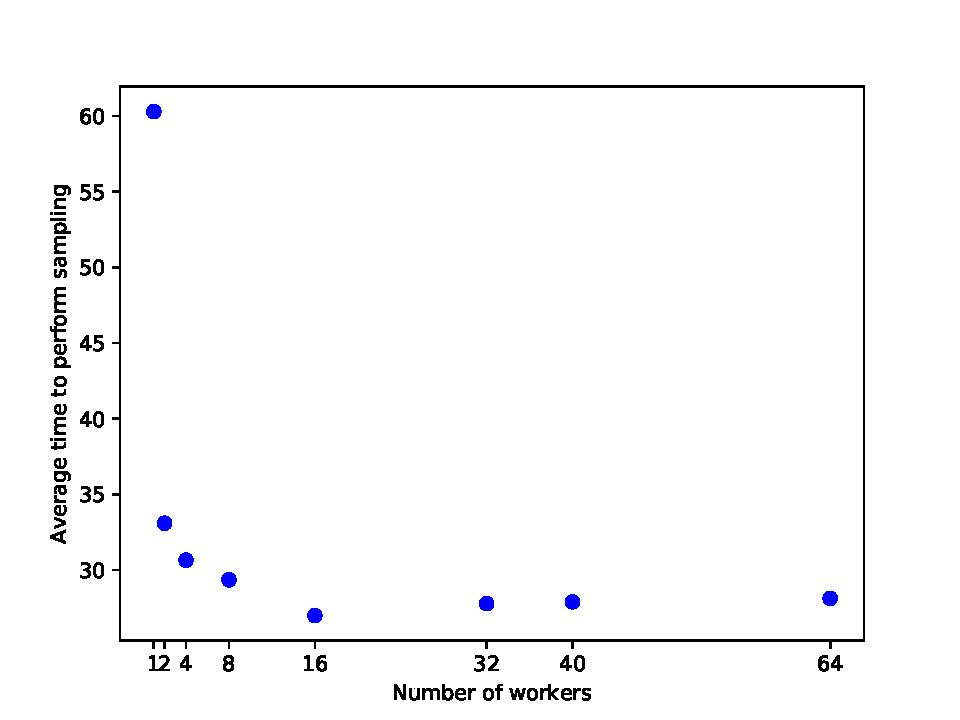
\includegraphics[width=.75\textwidth]{optimizations/workers_experiment.pdf}
    \caption{Average execution time of $500$ steps of the burn-in
        sampling, with varying number of workers. The average values are
        taken over 50 repetitions of the experiment. The model being
        sampled on this experiment contains 5 chemical reactions and 5
        chemical species.}
    \label{fig:parallel_map_sampling}
    \end{center}
\end{figure}

% Even after optimizing the sampling process of SigNetMS, we considered
% optimizing its use. Usually, we are not interested in running this
% software for one model only; the general use is to compare different
% models, and for this reason, we usually needed to run SigNetMS for
% multiple instances. In order to optimize this process, we created a
% program the runs SigNetMS with multiple instances, in a cluster. We
% call this program DistributedMS.
%
% DistributedMS receives as an input... 
% 
% To implement the distributed process, we used Rays library...

